\section{Résultats complémentaires}
\label{sec:S5}

\subsection{Caractéristiques de la base principale}
\label{sec:S5.1}

Cette configuration a été retenue au terme d'un essai préliminaire d'une quarantaine de configurations, sur un critère unique : le contraste entre politiques, sans lequel l'apprentissage causal n'aurait rien à identifier. La représentation par flux isole les mécanismes de capacité et rend les écarts entre politiques directement interprétables.

La base compte 2 000 scénarios, soit 8 000 versions de crise, et les cinq natures de perturbation y sont représentées de manière équilibrée (tableau~\ref{tab:d11}). La demande de référence, calibrée sur le volume encore livrable pendant l'incident (équation~\eqref{eq:S2}), est très faible lorsque la perturbation touche le hub de Nashville ou l'entrepôt d'Atlanta, par lesquels transite tout le flux : elle reflète la criticité du site touché autant que la taille du réseau.

\begin{table}[htbp]
\caption{Caractéristiques de la base principale.}
\label{tab:d11}
\footnotesize
\begin{tabularx}{\textwidth}{@{}LL@{}}
\toprule
\textbf{Caractéristique} & \textbf{Valeur} \\
\midrule
Scénarios ; versions de crise & 2 000 ; 8 000 \\
Répartition des natures & Panne fournisseur 422, fermeture d'un site de stockage 405, pic de demande 395, congestion 390, coupure de lien 388 \\
Durée de la perturbation, médiane [quartiles] & 16 jours [12 ; 20] \\
Sévérité, médiane [quartiles] & 0,91 [0,82 ; 0,95] \\
Part des articles critiques & 0,20 à 0,53 \\
Coefficient de détermination, médiane [quartiles] & 0,88 [0,79 ; 0,93] \\
Coefficient de détermination sur trajectoire lissée, médiane & 0,91 \\
Versions dont la chute est inférieure à 0,03 & 4,2 \% \\
Indicateurs non finis & 0 \\
Corrélation entre IPC et service perdu observé & 0,97 \\
\bottomrule
\end{tabularx}
\end{table}

L'ajustement est satisfaisant pour l'essentiel de la base : le coefficient de détermination médian atteint 0,88 et aucun indicateur n'est indéfini. Un quart des versions reste sous 0,8, principalement des crises courtes ou à reprise accidentée. L'indicateur de perte cumulée IPC reste néanmoins très fidèle au service effectivement perdu (corrélation de 0,97), ce qui justifie d'en faire l'indicateur principal de résilience : il dépend peu des imperfections de forme de la courbe ajustée.

\subsection{Effet des politiques selon la nature du choc et le réseau}
\label{sec:S5.2}

Les profils diffèrent aussi par les leviers engagés : le profil tardif n'engage que des leviers de demande, faute de pouvoir escalader au-delà de ses deux premiers choix pendant la crise, le profil prudent s'appuie surtout sur les stocks et la capacité additionnelle, le profil réactif sur le reroutage et la capacité. Leur efficacité dépend de la nature de la perturbation (tableau~\ref{tab:d13}).

\begin{table}[htbp]
\caption{Réduction médiane de la perte cumulée par rapport à l'absence de réaction, selon la nature de la perturbation.}
\label{tab:d13}
\footnotesize
\begin{tabularx}{\textwidth}{@{}LLLL@{}}
\toprule
\textbf{Nature} & \textbf{Réactif} & \textbf{Prudent} & \textbf{Tardif} \\
\midrule
Panne fournisseur & 84 \% & 0 \% & 0 \% \\
Coupure de lien & 73 \% & 17 \% & 0 \% \\
Fermeture d'un site de stockage & 82 \% & 10 \% & 2 \% \\
Pic de demande & 87 \% & 23 \% & 13 \% \\
Congestion & 78 \% & 41 \% & 15 \% \\
\bottomrule
\end{tabularx}
\end{table}

Le profil prudent est sans effet sur une panne fournisseur, que le déstockage ne compense pas, mais réduit de 41~\% la perte d'une congestion, choc diffus que des leviers globaux atténuent ; le profil réactif est le moins efficace face à une coupure de lien, dont les effets se propagent aux voies de secours.

Pour vérifier que ces résultats ne tiennent pas à la seule topologie d'ISOMORPH, un lot de contrôle de 500 scénarios a été généré sur le réseau paramétrique avec les mêmes réglages. Les crises y sont moins profondes (taux de service minimal médian de 0,91) et l'ajustement moins bon, mais la perte cumulée reste très fidèle au service perdu (corrélation de 0,97). Les grandes proportions sont remarquablement stables : la part du service perdu évitée atteint 67~\%, 17~\% et 13~\% pour les profils réactif, prudent et tardif, contre 73~\%, 18~\% et 14~\% sur ISOMORPH. La topologie modifie en revanche l'efficacité des leviers selon la nature du choc : sur le réseau paramétrique, dont les voies de secours sont de faible capacité, le profil réactif ne réduit plus que de 25~\% la perte d'une coupure de lien et de 53~\% celle d'une fermeture, contre 73~\% et 82~\% sur ISOMORPH. L'effet d'une politique dépend donc conjointement de la nature du choc et de la redondance du réseau.

\subsection{Pronostic, diagnostic et étude de cas}
\label{sec:S5.3}

Le pronostic, établi à partir des seules variables connues au moment de décider, classe correctement 65~\% des crises de test, contre 34~\% pour la classe majoritaire et 60~\% pour un modèle fondé sur la seule politique. Le gain apporté par le contexte est réel mais modeste. La courbe d'apprentissage est presque plate, de 62,5~\% avec 200 scénarios à 63,7~\% avec 1 600 : la taille de la base n'est pas le facteur limitant, c'est l'information disponible au moment de décider. La perte dépend notamment de la tension du réseau, que le générateur n'exporte pas.

Le diagnostic est bien calibré pour la politique et la durée. Pour les crises de test à forte perte, la probabilité a posteriori de chaque politique (sans réaction, tardif, prudent, réactif) vaut 0,42, 0,32, 0,26 et 0,01, pour des fréquences observées de 0,41, 0,33, 0,26 et 0,005 ; celle d'une perturbation longue vaut 0,41, comme sa fréquence observée. Il l'est moins pour la nature du choc et la position de la cible : les crises touchant un point de passage obligé, 6~\% de la base, sont trop rares pour que le score retienne leurs effets propres.

Deux crises de même nature illustrent l'usage du réseau. Dans la première, un site de stockage situé sur un point de passage obligé, comme l'entrepôt d'Atlanta, est fermé pour une longue durée. Le réseau (figure~\ref{fig:d7}) donne une probabilité de forte perte de 0,70 sans réaction, de 0,56 sous le profil tardif, de 0,44 sous le profil prudent et de 0,01 sous le profil réactif. Seul ce dernier atteint l'objectif avec une probabilité suffisante : la préconisation est sans ambiguïté, quel que soit le seuil retenu.

Dans la seconde, un site de stockage redondé est fermé pour une courte durée. La probabilité de forte perte tombe à 0,30 sans réaction, 0,22 sous le profil tardif et 0,20 sous le profil prudent. Avec $\theta$ = 0,8, le profil prudent atteint l'objectif avec une probabilité de 0,80 et devient la préconisation : face à un choc bref sur un site doublé, une réaction fondée sur le déstockage suffit, et mobiliser le reroutage et la capacité additionnelle n'apporterait qu'un gain marginal.

\begin{center}
% Figure : pronostic de la perte cumulée selon la politique (inférence dans BayesArtist sur le réseau appris)
% Évidences : nature = fermeture_entrepot, cible = passage_oblige, duree = fort ; valeurs lues dans BayesArtist.
\begin{tikzpicture}[x=1cm,y=1cm, font=\scriptsize]
  \node[anchor=east] at (-0.15,0.00) {Réactif};
  \fill[palmec!75] (0.000,-0.30) rectangle (10.812,0.30);
  \node at (5.406,0.00) {$0{,}90$};
  \fill[poltard!75] (10.812,-0.30) rectangle (11.904,0.30);
  \node at (11.358,0.00) {$0{,}09$};
  \fill[polprud!75] (11.904,-0.30) rectangle (11.988,0.30);
  \node[anchor=west] at (12.05,0.00) {$0{,}01$};
  \node[anchor=east] at (-0.15,-0.90) {Prudent};
  \fill[palmec!75] (0.000,-1.20) rectangle (1.272,-0.60);
  \node at (0.636,-0.90) {$0{,}11$};
  \fill[poltard!75] (1.272,-1.20) rectangle (6.672,-0.60);
  \node at (3.972,-0.90) {$0{,}45$};
  \fill[polprud!75] (6.672,-1.20) rectangle (12.000,-0.60);
  \node at (9.336,-0.90) {$0{,}44$};
  \node[anchor=east] at (-0.15,-1.80) {Tardif};
  \fill[palmec!75] (0.000,-2.10) rectangle (1.056,-1.50);
  \node at (0.528,-1.80) {$0{,}09$};
  \fill[poltard!75] (1.056,-2.10) rectangle (5.268,-1.50);
  \node at (3.162,-1.80) {$0{,}35$};
  \fill[polprud!75] (5.268,-2.10) rectangle (12.000,-1.50);
  \node at (8.634,-1.80) {$0{,}56$};
  \node[anchor=east] at (-0.15,-2.70) {Sans réaction};
  \fill[palmec!75] (0.000,-3.00) rectangle (0.816,-2.40);
  \node at (0.408,-2.70) {$0{,}07$};
  \fill[poltard!75] (0.816,-3.00) rectangle (3.600,-2.40);
  \node at (2.208,-2.70) {$0{,}23$};
  \fill[polprud!75] (3.600,-3.00) rectangle (12.000,-2.40);
  \node at (7.800,-2.70) {$0{,}70$};
  \draw[black!50] (0,-3.15) -- (12.0,-3.15);
  \foreach \p/\l in {0/0,0.2/0{,}2,0.4/0{,}4,0.6/0{,}6,0.8/0{,}8,1/1} { \draw[black!50] (\p*12.0,-3.15) -- ++(0,-0.08) node[below] {$\l$}; }
  \node[font=\small] at (6.0,-3.90) {Probabilité de chaque classe de perte cumulée IPC};
  \fill[palmec!75] (1.20,0.55) rectangle (1.55,0.8); \node[anchor=west] at (1.60,0.675) {Perte faible};
  \fill[poltard!75] (4.60,0.55) rectangle (4.95,0.8); \node[anchor=west] at (5.00,0.675) {Perte moyenne};
  \fill[polprud!75] (8.00,0.55) rectangle (8.35,0.8); \node[anchor=west] at (8.40,0.675) {Perte forte};
\end{tikzpicture}

\captionof{figure}{Pronostic de la perte cumulée selon la politique, pour la fermeture longue d'un site situé sur un point de passage obligé : distribution des trois classes d'IPC inférée par le réseau appris.}\label{fig:d7}
\end{center}

Le diagnostic éclaire le cas inverse, celui d'une crise à forte perte gérée par un profil prudent. Le réseau y associe une perturbation longue, avec une probabilité de 0,39 contre 0,33 a priori, un recours au déstockage presque certain (0,95) et une escalade jusqu'à trois leviers ou plus (0,40 contre 0,23 a priori). Il désigne ainsi une crise trop longue pour la politique choisie : le gestionnaire a escaladé, mais à partir de leviers de stock dont l'effet s'épuise, sans atteindre à temps le reroutage. Ce diagnostic oriente l'action corrective vers la politique, plus réactive ou dotée d'un autre ordre de leviers, plutôt que vers le réseau.

La figure~6 du manuscrit applique la lecture à rebours de la section~3.4 du manuscrit aux sept contextes que la topologie d'ISOMORPH rend possibles, pour l'objectif d'une perte cumulée faible. Le profil réactif est le plus probable partout, et d'autant plus que le choc dure : sa probabilité a posteriori passe de 0,51 à 0,58 pour un choc court à 0,72 à 0,79 pour un choc long. Pour un choc court, les trois autres politiques conservent chacune entre 0,12 et 0,18 : une perte faible y reste accessible sans réaction rapide, ce qui rejoint la préconisation sobre de la section~4.3 du manuscrit. La carte varie en revanche peu avec la nature du choc et la position de la cible, conformément au diagnostic : dans la structure apprise, ces variables n'agissent sur la perte qu'à travers les leviers mobilisés.

\subsection{Sensibilité à la couverture de stock}
\label{sec:S5.4}

La représentation temporelle permet d'étudier le rôle des stocks, que la base principale neutralise. Sur le réseau ISOMORPH, avec ses délais de trajet d'origine, 60 crises ont été simulées pour chaque nature de perturbation et chaque couverture, sans réaction du gestionnaire, et l'on a compté celles qui produisent une baisse de service visible (figure~\ref{fig:d8} et tableau~\ref{tab:S4}). La représentation par flux sert de référence.

\begin{center}
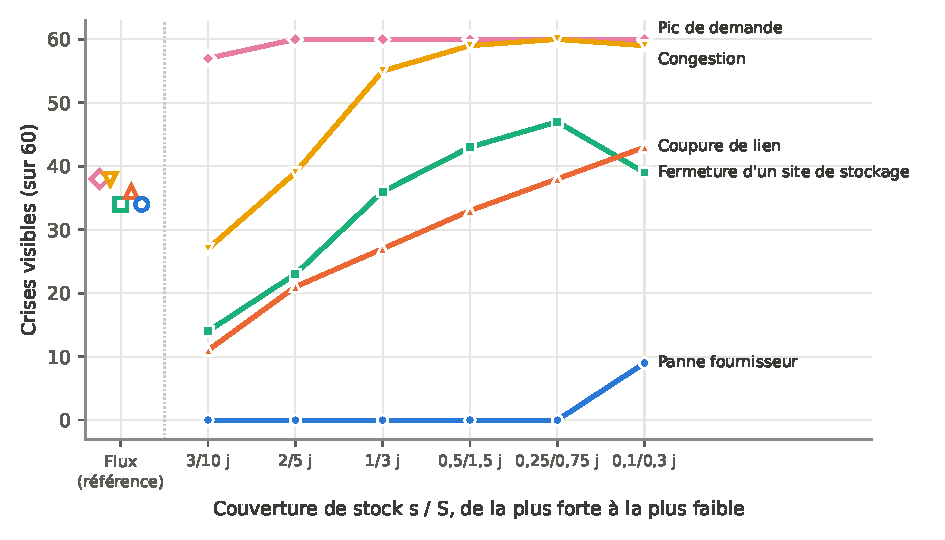
\includegraphics[width=0.75\textwidth]{figures/Fig8_couverture_stock.pdf}
\captionof{figure}{Nombre de crises visibles sur 60 selon la couverture de stock, par nature de perturbation (réseau ISOMORPH, sans réaction). Les symboles creux, à gauche, donnent la référence de la représentation par flux.}\label{fig:d8}
\end{center}

Pour les ruptures de distribution, coupure de lien, fermeture d'un site de stockage et congestion, la couverture agit comme un levier de robustesse progressif : plus elle est faible, plus les crises visibles sont nombreuses, de 11 à 43 sur 60 pour une coupure de lien et de 27 à 59 pour une congestion. La frontière entre robustesse et résilience évoquée en section~S3.3 se déplace donc de manière contrôlée avec le niveau de stock. Les pannes fournisseur sont au contraire absorbées dès que la couverture atteint un quart de jour, y compris pour des pannes de 15 à 60 jours à la couverture par défaut : la calibration de la demande borne le manque à servir pendant une panne, que quelques jours de stock suffisent à compenser. Enfin, le pic de demande est mieux absorbé sans stocks qu'avec : dans la représentation par flux, toute marge de capacité sert instantanément le surcroît de demande, alors qu'avec des délais, ce surcroît doit d'abord être prélevé sur des stocks dimensionnés sur le débit nominal, que le recomplètement ne reconstitue qu'après un délai.

La couverture de stock n'est donc pas un levier universel de résilience. Elle protège contre les pertes de capacité de distribution, est presque superflue contre une défaillance amont de faible ampleur, et ne protège pas contre un choc de demande, qui appelle des leviers de capacité ou de demande. Ces résultats, obtenus sans réaction du gestionnaire et à couverture uniforme, n'épuisent pas la question : l'interaction entre couverture et politique de gestion reste à étudier.

\begin{table}[htbp]
\caption{Crises produisant une baisse de service visible, sur 60, selon la couverture de stock (réseau ISOMORPH, sans réaction).}
\label{tab:S4}
\footnotesize
\begin{tabularx}{\textwidth}{@{}LLLLLLLL@{}}
\toprule
\textbf{Nature} & \textbf{Flux} & \textbf{3 / 10 j} & \textbf{2 / 5 j} & \textbf{1 / 3 j} & \textbf{0,5 / 1,5 j} & \textbf{0,25 / 0,75 j} & \textbf{0,1 / 0,3 j} \\
\midrule
Panne fournisseur & 34 & 0 & 0 & 0 & 0 & 0 & 9 \\
Coupure de lien & 36 & 11 & 21 & 27 & 33 & 38 & 43 \\
Fermeture d'un site de stockage & 34 & 14 & 23 & 36 & 43 & 47 & 39 \\
Pic de demande & 38 & 57 & 60 & 60 & 60 & 60 & 60 \\
Congestion & 38 & 27 & 39 & 55 & 59 & 60 & 59 \\
\bottomrule
\end{tabularx}
\end{table}

\subsection{Lecture économique détaillée et coût de la sur-réaction}
\label{sec:S5.5}

La politique réactive est à la fois la plus efficace et la plus rentable par levier : chacun de ses leviers préserve en moyenne 6 630 unités, soit environ un tiers de journée de demande. Pour une marge de 10 euros par unité, elle reste rentable tant qu'un levier coûte moins de 66 000 euros par crise. La politique prudente est au contraire économiquement dominée : elle engage plus des deux tiers des leviers de la politique réactive pour un quart de ses gains, et chaque levier qu'elle ajoute à la politique tardive ne préserve que 790 unités. Le coût d'une politique tient donc moins au nombre de leviers qu'à leur moment d'engagement : engagés tôt, ils évitent l'allongement de la crise ; engagés tard ou dans le mauvais ordre, ils arrivent quand l'essentiel de la perte est consommé. La rentabilité dépend aussi de la nature du choc : le seuil de la politique réactive atteint 13 100 unités par levier pour une panne fournisseur, mais seulement 2 300 pour une congestion, que des leviers globaux atténuent mal. Le seuil élevé de la politique tardive appelle une réserve : ses gains viennent surtout des leviers de demande, et en particulier du report de la demande non critique, qui relève le taux de service mesuré en différant des ventes plutôt qu'en les préservant. Une partie de ces gains est donc reportée sur la période suivante, et son seuil de rentabilité est probablement surestimé.

La figure~7 du manuscrit en tire la conséquence pour le choix d'une politique. Parmi les politiques fixes, la réactivité est optimale tant que le coût d'un levier reste sous le seuil de 6 630 unités de marge ; au-delà, mieux vaut ne pas réagir, et les politiques prudente et tardive ne sont jamais le meilleur choix. La courbe noire en tirets retient, pour chaque crise et chaque coût de levier, la politique au meilleur bénéfice, puis en fait la moyenne sur les 2 000 crises. Ce choix est fait a posteriori, comme si l'issue de chaque politique était connue d'avance : la courbe constitue donc une limite haute de ce qu'une préconisation adaptée à la crise peut rapporter, dont le réseau bayésien, qui ne connaît la crise que partiellement, ne capte qu'une partie. Cette limite haute conserve un bénéfice positif bien au-delà du seuil de la politique réactive, parce que pour certaines crises la politique tardive ou l'absence de réaction suffisent. Pour un levier valant 5 000 unités de marge, le choix adapté porterait le bénéfice moyen de 4 560 à 8 350 unités par crise, soit 83~\% de plus que la meilleure politique fixe ; pour un levier plus coûteux, il resterait le seul à dégager un gain. C'est la valeur économique que vise la préconisation du réseau bayésien : identifier, à partir de ce que l'on sait de la crise, celles où une politique plus sobre suffit.

Deux lots complémentaires, aux réglages du lot principal, mesurent le coût de la sur-réaction : 400 scénarios sans perturbation perceptible et 300 perturbations mineures (sévérité de 0,1 à 0,3, durée de 1 à 3 jours). Sans perturbation, aucun profil n'engage de levier : la détection, fondée sur le taux de service lissé, ne se déclenche pas sur les seules fluctuations de la demande. Face à une perturbation mineure, en revanche, le profil réactif engage au moins un levier dans 32~\% des cas, contre 4~\% pour le profil prudent et aucun pour le profil tardif, pour ne réduire les ventes perdues que de 2 335 à 2 260 unités par crise. Chaque levier y préserve environ 230 unités, près de trente fois moins que sur l'ensemble des crises de la base principale. La sensibilité du profil réactif a donc un coût réel face aux chocs mineurs, pour l'essentiel des pics de demande et des congestions : elle ne se justifie que si l'on sait distinguer un choc mineur d'une crise sévère, ce que vise le pronostic du réseau bayésien.
